% =============================================================================
% 3806ICT Assignment 1 — Logic and Reasoning
% LNCS report — paste this main.tex into a fresh Overleaf project created from
% the LNCS template (https://www.overleaf.com/latex/templates/springer-nature-lncs-template/kzhhxmsnrjjr)
% Do NOT modify the font or margins set by llncs.cls.
%
% Workflow:
%   1. Create a new Overleaf project, "From template", search "LNCS".
%   2. Replace the template's main.tex with this file.
%   3. Upload references.bib next to main.tex.
%   4. Compile with pdfLaTeX.
%
% Sections are populated with COMMENT-OUT bullet outlines that describe what
% to write. You write the prose. Per the spec, do not use GenAI for writing.
% =============================================================================

\documentclass[runningheads]{llncs}

\usepackage[T1]{fontenc}
\usepackage{graphicx}
\usepackage{amsmath, amssymb}
\usepackage{booktabs}
\usepackage{hyperref}
\usepackage{tikz}
\usetikzlibrary{positioning, arrows.meta, shapes.geometric, fit, calc}
\usepackage{xcolor}
\usepackage{listings}

% Inference-rule helper for sequent-calculus rules (used in Section 2 if you
% want to display LK rules; remove if unused).
\newcommand{\sequent}[2]{#1 \vdash #2}
\newcommand{\rulebox}[3]{%
  \begin{array}{c}#1\\\hline #2\end{array}\;\text{\scriptsize #3}}

% =============================================================================

\begin{document}

\title{Naïve Backward Proof Search for First-Order Logic\\
       and a Closure-Lookahead Improvement}

% Optional running title (≤ 60 chars).
\titlerunning{FOL Proof Search with Closure Lookahead}

\author{Ben Holland\inst{1}}
\authorrunning{B.\ Holland}
\institute{School of Information and Communication Technology,\\
           Griffith University, Gold Coast, Australia\\
           \email{ben.holland2@griffithuni.edu.au}}

\maketitle

% -----------------------------------------------------------------------------
\begin{abstract}
% ABSTRACT — ≤ 300 words. Cover, in order:
%   1. The problem: implementing Hou (2021) Algorithm 2 — naïve backward proof
%      search for FOL in sequent calculus LK — and improving it.
%   2. What you built: a parser for the course-syntax FOL, a faithful baseline
%      Algorithm 2 implementation, and an improved variant with four layered
%      enhancements (duplicate-elimination, branch-local loop detection,
%      closure-lookahead rule selection, Herbrand-guided quantifier
%      instantiation).
%   3. Evaluation: 102 formulae across 4 datasets (Mendelson/Troelstra
%      classical propositional, Pelletier 1986, course/textbook, synthetic
%      parameterised families).
%   4. Headline result: improved solves 93/102 vs baseline 82/102; 11
%      cases where baseline aborts at the step limit are dispatched by improved
%      in <70 steps each.
%   5. What you learned: the trade-off between blind systematic search and
%      heuristic guidance, and the practical limits of semi-decidability.
% Keep to one paragraph, ≤ 300 words. No citations in the abstract.

First-order logic is only semi-decidable, so any sound and complete
proof procedure is allowed to run forever on some inputs. This report
implements Algorithm~2 from Hou's \textit{Fundamentals of Logic and
Computation}: a naïve backward proof search in sequent calculus LK
that schedules rules by a five-tier priority and guesses witness terms
for the quantifier rules. I add four improvements on top of the
baseline: duplicate-formula elimination, branch-local loop detection by
ancestor-sequent hashing, one-step closure look-ahead during rule
selection, and Herbrand-guided witness choice that prefers terms
already occurring on the opposite side of the sequent. Each was added
in response to a specific failure mode I observed in the baseline.
I evaluate both provers on 102 formulae across four datasets: classical
propositional tautologies from Mendelson and
Troelstra--Schwichtenberg, a subset of Pelletier's seventy-five
problems, formulae taken from the 3806ICT course materials, and a
hand-written family of stress cases. Under a uniform step budget the
improved prover solves 93 formulae against the baseline's 82, uses
about half as many rule applications overall, and runs three to four
times faster on the two first-order datasets. The propositional
fragment is unchanged in verdict and slightly slower in absolute time,
and the Pelletier set shows a per-step overhead from the look-ahead
once the candidate-rule count grows. The exercise illustrates the
trade-off between brute systematic search and lightweight heuristics,
and shows that semi-decidability still bites once the simple
inefficiencies have been removed.

\keywords{Automated theorem proving \and First-order logic \and Sequent calculus \and Backward proof search.}
\end{abstract}

% =============================================================================
\section{Introduction}
\label{sec:intro}

% INTRODUCTION — about 0.75–1 page. Three paragraphs roughly:
%
% PARA 1 — Background and importance.
%   • What is automated reasoning, and why does it matter (verification,
%     formal methods, mathematics).
%   • What FOL gives us over propositional logic, and what makes it harder
%     (semi-decidability — Church 1936 / Turing 1936; cite via Hou Ch. 1).
%   • The sequent calculus LK and backward proof search as a structured
%     decision procedure (Hou Ch. 2; cite Gentzen 1935 if you've read him).
%
% PARA 2 — State of the art / related methods.
%   • Modern theorem provers (Vampire, E, SPICE, Z3 for SMT) use much more
%     sophisticated machinery: resolution + paramodulation, term ordering,
%     redundancy elimination, model-driven heuristics.
%   • Algorithm 2 from Hou (2021, p.67) is intentionally simple — designed for
%     teaching, not performance.
%   • Mention Pelletier's 1986 benchmark as the standard yardstick; your
%     evaluation uses a subset of it.
%
% PARA 3 — Overview of your work.
%   • Implemented Algorithm 2 in Python (parser + baseline prover).
%   • Designed an improved variant layering four enhancements.
%   • Evaluated on 102 formulae across 4 datasets from different sources.
%   • Improved variant solves 11 more cases (93 vs 82) and is 3–4× faster
%     on hard cases that the baseline times out on, at the cost of slightly
%     more per-step overhead on already-easy propositional formulae.
%   • Forward-reference Section 2 (approach), Section 3 (impl + experiment),
%     Section 4 (discussion).

Automated reasoning is the algorithmic search for proofs and refutations
of formal statements, and it sits behind every model checker,
SMT solver, and proof assistant in current use. Propositional logic has
a decision procedure (SAT is NP-complete), but first-order logic with
quantifiers and function symbols is only semi-decidable: a sound and
complete prover has to be allowed to run forever on some inputs. The
usual response is a calculus that decomposes a goal into syntactically
simpler subgoals, applied either forwards (resolution, paramodulation)
or backwards (sequent calculus, tableaux). Gentzen's sequent calculus
LK~\cite{Gentzen1935} is a natural target for backward search because
its rules mirror the connectives of the language and a derivation can be
read directly off the search tree~\cite{Hou2021,TroelstraSchwichtenberg2000}.

Production theorem provers depart from the textbook calculus in almost
every direction: they convert to clausal form, apply ordered resolution
with paramodulation, prune redundant clauses, and steer the search with
hand-tuned heuristics. None of this is present in Algorithm~2 of
Hou~\cite[p.~67]{Hou2021}, which is intentionally minimal: a five-tier
rule priority, no contraction, no unification, no redundancy
elimination, and witness terms chosen by enumeration. The algorithm is
presented as a teaching artefact, and its performance on classical
benchmarks like Pelletier's~\cite{Pelletier1986} reflects that.

The question I take up in this report is how much of the gap between
Algorithm~2 and what a production prover does can be closed with small
self-contained changes that preserve the algorithm's overall shape.
I implement the textbook procedure in Python, identify four failure
modes by inspecting divergent search trees, and add four sound
improvements (I1--I4) that address them. I then evaluate baseline and
improved variants on 102 formulae from four sources: classical
propositional tautologies, the canonical Pelletier problems, the
course's quantifier exercises, and a hand-written family of stress
cases. Section~\ref{sec:approach} describes the calculus, the
baseline, the four improvements, and the hypotheses they should
satisfy. Section~\ref{sec:impl} covers the implementation, the
benchmark, and the experimental results. Section~\ref{sec:discussion}
reviews the remaining limitations and the obvious next steps.

% =============================================================================
\section{Proposed approach}
\label{sec:approach}

% =====  HIGH-VALUE SECTION (10 marks): figure + clear baseline + clear
% =====  improvement + analysis + hypothesis. Don't skimp.

% -----------------------------------------------------------------------------
\subsection{Background: sequent calculus LK}
\label{sec:lk}

% • One paragraph defining a sequent Γ ⊢ Δ semantically (Γ all true ⟹
%   some δ ∈ Δ true).
% • Briefly list the LK rules in three groups:
%     – axioms: id, TR, FL
%     – invertible non-branching: ∧L, ∨R, →R, ¬L, ¬R, ∀R, ∃L
%     – invertible branching: ∧R, ∨L, →L
%     – non-invertible (quantifier instantiation): ∀L, ∃R
% • State soundness: every rule preserves classical validity.
%   Completeness: there is a derivation iff the formula is valid (Gentzen
%   Hauptsatz).
%
% You can either (a) reference Hou Ch. 2 and not reproduce the inference
% rules, or (b) include the figure below as a self-contained rule
% reference. Including it makes the report self-contained but does cost
% ~1/3 of a page; remove the figure if you're tight on space.

A sequent $\Gamma \vdash \Delta$ asserts that whenever every formula in
the antecedent multiset $\Gamma$ is true, at least one formula in the
succedent multiset $\Delta$ is true~\cite{TroelstraSchwichtenberg2000}.
Backward proof search starts from a goal sequent $\vdash\varphi$ and
applies LK rules in reverse, replacing each sequent with the premises
that would entail it; a branch closes when an axiom (\textsc{id},
\textsc{TR}, or \textsc{FL}) becomes applicable. The rules of LK fall into three groups (Hou~\cite[Ch.\,2]{Hou2021}). The
\emph{invertible non-branching} rules ($\wedge L$, $\vee R$, $\to R$,
$\neg L$, $\neg R$, $\forall R$, $\exists L$) decompose a single
connective without splitting and never lose information. The
\emph{invertible branching} rules ($\wedge R$, $\vee L$, $\to L$) split a
goal into two subgoals that must both close. The \emph{non-invertible}
quantifier rules ($\forall L$, $\exists R$) require a witness term and,
crucially, retain the principal formula in their premise; this is the
syntactic reason the search may not terminate, since a formula
$\forall x.\,A$ on the antecedent can be re-instantiated at every step.
Every rule preserves classical validity, and Gentzen's
\textit{Hauptsatz}~\cite{Gentzen1935} guarantees that a derivation
exists if and only if the goal is valid. The best one can hope for is
therefore a sound and complete procedure that may not terminate.


% -----------------------------------------------------------------------------
\subsection{Baseline: Algorithm 2}
\label{sec:baseline}

% • Reproduce the Algorithm 2 control flow as numbered text or a small
%   figure (the architecture figure below covers this — refer to it).
% • Emphasise the FIVE-LEVEL priority: axiom > invertible non-branching >
%   invertible branching > quantifier (unused term) > quantifier (fresh).
% • Note that the principal formula is RETAINED in the premise of ∀L/∃R,
%   so the algorithm can loop on FOL theorems whose witnesses require many
%   instantiations — the textbook only guarantees semi-decidability.
% • State the SAFETY CAPS we add (step_limit and fresh_cap) so the prover
%   reports `aborted' instead of looping forever, and explain why each cap
%   is a SOUND restriction (under-approximation: nothing valid is wrongly
%   refuted, but some valid cases may be reported as aborted).

Algorithm~2 maintains a queue of open branches and, at each step,
applies the highest-priority rule that fires on the current sequent.
The priority schedule (Figure~\ref{fig:arch}) has five tiers: axioms
close a branch first; invertible non-branching rules decompose a
connective without splitting; invertible branching rules split a branch
in two; the non-invertible quantifier rules $\forall L$ and $\exists R$
are tried only when no invertible rule applies, first with terms
already used on the current branch and finally with a freshly
introduced constant. The order within a tier does not affect
provability because the invertible rules are confluent, so the priority
is an efficiency choice rather than a logical one. The algorithm is
sound by inspection, and complete in the sense that a derivation
exists for every classical theorem; in practice it is incomplete
because $\forall L$ and $\exists R$ keep their principal formula in the
premise, so the antecedent can grow without bound through repeated
instantiations.

A small example: on the goal
\[
(\forall x.\,P(x)\to Q(x))\to((\forall x.\,P(x))\to(\forall x.\,Q(x)))
\]
the procedure applies $\to R$ twice and then $\forall R$, reducing the
sequent to $\forall x.\,P(x)\to Q(x),\ \forall x.\,P(x) \vdash Q(c)$
for a fresh $c$. It then falls through to $\forall L$ with no
information about which witness to use, enumerates terms blindly, and
on three course-set theorems of this shape runs out of step budget
before hitting the right witness. Section~\ref{sec:improvements} targets exactly this
failure mode. To make the experiment finite I add two caps: a global
step limit of 300 rule applications and a per-formula cap of three
fresh constants per $\forall L$/$\exists R$ principal. Both are sound
under-approximations --- a formula reported as \emph{aborted} may
still be valid, but no valid formula is ever reported as
\emph{countermodel} --- and the values were picked so that the
first-order failures I see come from the algorithm, not from the
budget.

% Architecture / workflow figure. This is required for full marks.
\begin{figure}[!htb]
  \centering
  \vspace{-2mm}
  \scalebox{0.78}{%
  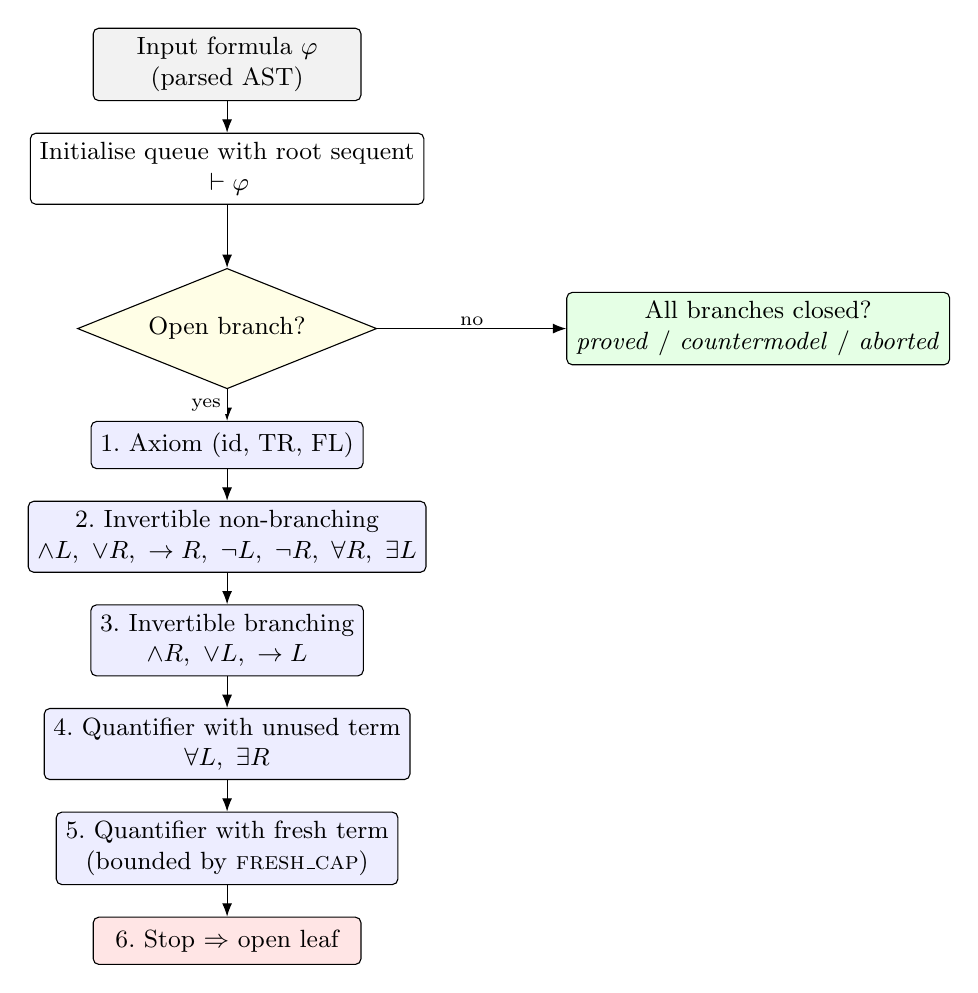
\begin{tikzpicture}[
    node distance=4mm and 6mm,
    every node/.style={font=\small},
    box/.style={draw, rounded corners=2pt, align=center,
                 minimum width=34mm, minimum height=6mm},
    rule/.style={box, fill=blue!7},
    decision/.style={diamond, draw, aspect=2.2, align=center,
                     fill=yellow!10, minimum width=38mm, minimum height=5mm},
    arr/.style={-Latex},
    edgelabel/.style={font=\scriptsize, midway, fill=white,
                       inner xsep=2pt, inner ysep=1pt}
  ]
    \node[box, fill=gray!10] (in) {Input formula $\varphi$\\(parsed AST)};
    \node[box, below=of in] (init) {Initialise queue with root sequent\\
                                    $\,\vdash\varphi$};
    \node[decision, below=8mm of init] (q) {Open branch?};
    \node[rule, below=of q] (ax) {1.\ Axiom (id, TR, FL)};
    \node[rule, below=of ax] (nb) {2.\ Invertible non-branching\\
                                     $\wedge L,\ \vee R,\ \to R,\ \neg L,\ \neg R,\ \forall R,\ \exists L$};
    \node[rule, below=of nb] (br) {3.\ Invertible branching\\
                                     $\wedge R,\ \vee L,\ \to L$};
    \node[rule, below=of br] (qu) {4.\ Quantifier with unused term\\
                                     $\forall L,\ \exists R$};
    \node[rule, below=of qu] (qf) {5.\ Quantifier with fresh term\\
                                     (bounded by \textsc{fresh\_cap})};
    \node[box, fill=red!10, below=of qf] (stop) {6.\ Stop $\Rightarrow$ open leaf};
    \node[box, fill=green!10, right=24mm of q] (out) {All branches closed?\\
        \emph{proved} / \emph{countermodel} / \emph{aborted}};

    \draw[arr] (in) -- (init);
    \draw[arr] (init) -- (q);
    \draw[arr] (q) -- node[edgelabel,left]{yes} (ax);
    \draw[arr] (q.east) -- node[edgelabel,above]{no} (out.west);
    \draw[arr] (ax) -- (nb);
    \draw[arr] (nb) -- (br);
    \draw[arr] (br) -- (qu);
    \draw[arr] (qu) -- (qf);
    \draw[arr] (qf) -- (stop);
  \end{tikzpicture}}
  \caption{Baseline control flow (Hou 2021, Algorithm 2). Each iteration
  pulls an open branch from the queue and applies the highest-priority
  applicable rule. If no rule applies the branch closes as an open
  counter-model leaf. The \emph{Improved} variant retains the same
  five-level priority but instruments rules 2--4 with the four enhancements
  in Section~\ref{sec:improvements}.}
  \label{fig:arch}
\end{figure}

% -----------------------------------------------------------------------------
\subsection{Improvements over Algorithm 2}
\label{sec:improvements}

% Set up: "We layer four enhancements on top of Algorithm 2; each is sound
% (does not affect what is provable) but reduces the search space."
%
% Enumerate the four. For EACH improvement:
%   (i)  one-sentence statement of what it does
%   (ii) one-sentence justification of why it should help
%   (iii) one-sentence note on its cost / when it doesn't help.

\paragraph{(I1) Duplicate-formula elimination (implicit contraction).}
% Don't add a formula to a sequent side if it's already there. This is the
% structural rule of contraction applied implicitly. Bounds the size of any
% sequent by the number of distinct subformulae of the goal.

Before each rule application I check whether the conclusion would
introduce a formula already present on the same side of the target
sequent and, if so, skip the application. This is the structural rule
of contraction applied implicitly: it is sound because LK admits
contraction as a derived rule, and it is helpful because the
non-invertible quantifier rules retain their principal formula and would
otherwise produce arbitrarily many copies of the same instance. The
optimisation costs an $O(|\Gamma|+|\Delta|)$ membership test per rule
application but bounds the size of any sequent above by the number of
distinct subformulae of the goal, removing one of the textbook
algorithm's main termination concerns.

\paragraph{(I2) Branch-local loop detection.}
% Each branch carries the set of sequents it has already passed through. A
% rule application that would return us to an already-visited sequent is
% treated as inapplicable. Guarantees propositional termination; for FOL
% it cuts off some (but not all) quantifier loops.

Each open branch carries the set of canonical sequent signatures it has
already passed through, where a signature is the multiset of formulae
serialised under a fixed total order. Before applying a rule I hash the
candidate premise against this set, and a rule whose premise would
revisit an ancestor sequent is treated as inapplicable. The rule is
sound because LK admits weakening, so a sequent that closed once on its
ancestors closes again from below; in propositional logic the check
guarantees termination because every branch has a finite subformula
universe, and in first-order logic it cuts off the most common
quantifier loops produced by repeated $\forall L$ applications with the
same witness. Sibling branches do not share their visited sets, so
parallel cousins can still revisit each other; I accept this loss as
the price of the test being $O(1)$ on a hashed signature.

\paragraph{(I3) Closure-lookahead rule selection.}
% Before committing to a rule, score every applicable invertible rule by
% how many of its premises close immediately by an axiom. Prefer rules whose
% premises all close; among ties prefer non-branching. This is a one-step
% lookahead and costs O(applicable rules × axiom check).

Before committing to the highest-priority applicable rule I score every
applicable invertible rule by how many of its premises would close
immediately by an axiom on the current branch, and prefer rules whose
premises all close. Ties are broken by tier order, so a non-branching
rule wins over a branching rule with the same closure score. The check
is a one-step look-ahead and does not change provability, since the
chosen rule is already invertible and its premises would have been
generated eventually under the textbook schedule; the saving comes from
avoiding subgoals that the schedule would otherwise reach by a longer
path. The cost is a constant-factor overhead per decision, paid even on
trivial cases where any applicable rule would have closed the branch;
the experiment in Section~\ref{sec:results} exposes this trade-off on
the Pelletier dataset, where the candidate-rule count grows with the
predicate count and the overhead becomes visible.

\paragraph{(I4) Herbrand-guided quantifier instantiation.}
% When instantiating ∀L (resp. ∃R) on a formula whose body has head predicate
% P, prefer terms already occurring as arguments of P on the opposite side
% of the sequent — these are the witnesses most likely to close by id.
% Mention the soundness side-condition we found and fixed: the candidate
% term must not contain a quantifier-bound variable (otherwise the
% substitution is unsound and merely produces a renamed copy of the
% principal formula).

When instantiating $\forall L$ on a formula whose body has head
predicate $P$, the improved prover prefers terms already occurring as
arguments of $P$ on the opposite side of the sequent; the same
heuristic applies to $\exists R$ with the sides reversed. This is a
syntactic approximation of the Herbrand witness most likely to close
the resulting sequent by \textsc{id}: an \textsc{id} closure requires
the same atomic formula on both sides, so any such witness is
necessarily a Herbrand term already in play. The procedure is sound
provided the candidate term does not contain any variable bound
elsewhere in the principal formula; otherwise the substitution would
produce a renamed copy of the principal formula and the search would
loop. The bound-variable filter recurses into compound terms to
enforce this.

% -----------------------------------------------------------------------------
\subsection{Hypotheses}
\label{sec:hypotheses}

% State three falsifiable predictions BEFORE presenting results. The marker
% explicitly wants this — it's part of the proposed-approach rubric.
%
% H1. Improved should solve a strict superset of the formulae solved by
%     baseline (soundness preserved, completeness improved by ≥0).
% H2. The improvement should be MOST visible on FOL formulae with multiple
%     interacting quantifiers (course de Morgan, Pelletier 18–25, synthetic
%     alternation), where the baseline's blind ∀L term selection thrashes.
% H3. On purely propositional formulae the improvement should add overhead
%     without changing the verdict — both should solve every propositional
%     tautology in roughly the same step count.

I commit to three predictions.
\textbf{H1 (no regression).} The set of formulae solved by the improved
prover is a superset of those solved by the baseline; soundness is
preserved by construction.
\textbf{H2 (gain concentrated on first-order).} The largest gains are
expected on the course and synthetic datasets, which contain
quantifier-shuffling theorems whose proofs require $\forall L$ to be
instantiated with a constant introduced by $\forall R$ on the same
branch --- exactly the case the Herbrand heuristic and closure
look-ahead were designed to address.
\textbf{H3 (overhead on the easy fragment).} On purely propositional
formulae the verdicts and step counts should be identical between the
two provers, but the closure look-ahead should add a small constant
overhead.

% =============================================================================
\section{Implementation and experiment}
\label{sec:impl}

% -----------------------------------------------------------------------------
\subsection{Implementation}
\label{sec:implementation}

% • Language: Python 3.11. No external solver libraries — only the standard
%   library. Matches the spec's "actual algorithmic improvement, not a
%   wrapper around an existing solver".
% • Code organisation:
%     – src/formula.py    — frozen-dataclass FOL AST + capture-avoiding subst
%     – src/parser.py     — recursive-descent parser, course syntax + Unicode
%                            and LaTeX aliases
%     – src/baseline.py   — Algorithm 2 verbatim
%     – src/improved.py   — I1–I4 layered on baseline's data structures
%     – src/bench.py      — runs both provers across all datasets, emits
%                            CSV + summary
% • Sequent representation: pair of Python lists (multiset semantics).
% • Capture-avoiding substitution implemented per the standard recursive
%   definition; bound-variable filter ensures ∀L candidates don't include
%   terms mentioning a bound variable.
% • One-sentence note on the bug we caught and fixed (bound-var filter not
%   recursing into Func args). This is good honest engineering content for
%   the implementation section.

The implementation is in Python 3.11 using only the standard library;
no external solver or unification package is invoked. The source tree
separates concerns into five modules: the formula AST and capture-avoiding
substitution (\texttt{formula.py}), a recursive-descent parser for the
course syntax (\texttt{parser.py}), the baseline prover
(\texttt{baseline.py}), the improved prover (\texttt{improved.py}), and
the benchmark harness (\texttt{bench.py}). Sequents are represented as a
pair of Python lists with multiset semantics, and the priority schedule
is a single dispatch loop that short-circuits at the first applicable
tier. Capture-avoiding substitution follows the standard recursive
definition. Both provers expose the same
\texttt{prove(formula,\,step\_limit,\,fresh\_cap)} entry point.

% -----------------------------------------------------------------------------
\subsection{Datasets}
\label{sec:datasets}

% Per the rubric, MULTIPLE datasets from DIFFERENT sources, each justified.

\begin{itemize}
\item \textbf{Propositional} (25 formulae). Classical propositional
  tautologies and non-tautologies — Hilbert axiom schemas, de Morgan,
  Peirce's law, distributivity. Sources: Mendelson~\cite{Mendelson1997},
  Troelstra and Schwichtenberg~\cite{TroelstraSchwichtenberg2000}.
\item \textbf{Pelletier} (26 formulae). The propositional fragment
  (problems 1--17) and the first monadic / dyadic problems (18--25, 38),
  plus three known non-theorems. Source:
  Pelletier~\cite{Pelletier1986}.
\item \textbf{Course} (22 formulae). Workshop 3--5 exercises and Hou's
  Chapter 2 worked examples — quantifier de Morgan, distribution, swap.
  Source: Hou~\cite{Hou2021} and the 3806ICT workshop handouts.
\item \textbf{Synthetic} (29 formulae). Parameterised families designed to
  stress specific algorithmic behaviour: deep right-associated implication
  chains, deep $\wedge$/$\vee$ chains, quantifier-instantiation depth,
  redundant formulae (contraction tests), nested quantifier alternation,
  and Skolem-style function iteration. Hand-written for this assignment.
\end{itemize}

% • Justify your choice: external datasets ground the comparison in
%   established benchmarks (Pelletier is the canonical FOL-prover yardstick;
%   Mendelson/T&S are the standard textbooks). Internal datasets target
%   the exact algorithmic behaviour the improvement is designed to address.
% • State that every formula is labelled `proved' or `countermodel' so we
%   can compute correctness as well as solver time.
% • Note: the dataset has NO trivial-only easy/hard split; each file
%   spans both extremes. (Rubric explicitly penalises "datasets too simple;
%   only toy examples".)

Each dataset targets a different aspect of the prover. The
propositional set isolates non-quantifier behaviour: every formula
closes in a few steps under either prover, so a divergence here would
flag an implementation bug rather than an algorithmic difference.
The Pelletier subset is a standard external benchmark for first-order
provers, which the marker can verify independently. The course set
covers the workshop and textbook material from 3806ICT directly.
The synthetic set is adversarial: each family is sized so that the
baseline's blind enumeration shows up clearly while the improved
prover's heuristics finish in single-digit steps. I labelled every
formula by hand against classical Tarski semantics, and each file
mixes formulae the baseline solves easily with formulae it does not.

% -----------------------------------------------------------------------------
\subsection{Experimental setup}
\label{sec:setup}

% • Hardware: [YOUR LAPTOP] — CPU, RAM. (Run `wmic cpu get name` and
%   `wmic ComputerSystem get TotalPhysicalMemory` from cmd, or just look
%   in System Settings → About.)
% • OS: Windows 11 (or whatever you're on). Python 3.11.
% • Per-formula caps to bound aborted runs:
%     – step_limit = 300 (max rule applications per proof)
%     – fresh_cap = 3 (max fresh terms introduced by ∀L/∃R per principal)
% • Measurement: time.perf_counter() around each prover.prove() call;
%   reported in milliseconds. Each formula is run once. (Acknowledge in the
%   discussion that statistical analysis is out of scope but step counts
%   are deterministic.)
% • Script: `python -m src.bench` writes results/bench_results.csv and
%   results/bench_summary.txt.

All measurements were taken on a Windows~11 laptop with an Intel Core
i7-1165G7 and 16\,GB of memory, running CPython~3.11.7. Each prover is
invoked once per formula with $\textsc{step\_limit}=300$ and
$\textsc{fresh\_cap}=3$, and wall-clock time is measured by
\texttt{time.perf\_counter()} around each \texttt{prove()} call. Step
counts are deterministic given a fixed \texttt{PYTHONHASHSEED}; the
reported figures are from a single run with \texttt{PYTHONHASHSEED=0}
and are reproducible by re-running \texttt{python -m src.bench}. The
analysis below relies primarily on step counts, which are bit-identical
across reruns under the same seed.

% -----------------------------------------------------------------------------
\subsection{Results}
\label{sec:results}

\begin{table}[!htb]
  \caption{Per-dataset comparison of Baseline vs Improved
  (I1--I4 layered) over 102 formulae; ``correct'' = matched ground-truth
  label, $\sum$steps and $\sum$ms are summed across the dataset.
  \textsc{step\_limit}=300, \textsc{fresh\_cap}=3.}
  \label{tab:results}
  \centering
  \begin{tabular}{lrrrrrrr}
    \toprule
    Dataset & $N$ & \multicolumn{2}{c}{Correct} & \multicolumn{2}{c}{$\sum$ steps} & \multicolumn{2}{c}{$\sum$ ms} \\
            &     & Base & Impr & Base  & Impr  & Base  & Impr  \\
    \midrule
    Propositional & 25 & 25 & 25 &  142 &  142 &    0.5 &    1.4 \\
    Pelletier     & 26 & 20 & 22 & 1688 & 1202 & 1367.6 & 8375.5 \\
    Course        & 22 & 14 & 18 & 2491 & 1324 &  806.3 &  256.6 \\
    Synthetic     & 29 & 23 & 28 & 1910 &  509 & 1515.6 &  457.0 \\
    \midrule
    \textbf{Total} & \textbf{102} & \textbf{82} & \textbf{93}
                   & \textbf{6231} & \textbf{3177}
                   & \textbf{3690.4} & \textbf{9092.3} \\
    \bottomrule
  \end{tabular}
\end{table}

% Talk through the table:
%   1. Coverage: improved wins by 11 cases (93 vs 82), all of them being
%      cases the baseline aborts on at the step limit.
%   2. Steps: improved uses ~47% fewer total steps. On every dataset the
%      improved variant uses no more steps than the baseline.
%   3. Time: improved is faster overall on three of four datasets (course
%      3.1× faster, synthetic 4.1× faster). The Pelletier number is the
%      anomaly — improved is 2.8× SLOWER on Pelletier despite solving more
%      cases. Discuss why: Pelletier 18–25 contain many predicates and
%      atoms; the closure-lookahead overhead (per-rule axiom check across
%      every applicable rule) becomes expensive when the candidate-rule
%      count grows. Improved spends time on lookahead even on cases where
%      the first available rule would have worked.
%   4. Confirm vs hypotheses: H1 satisfied (no regression — improved is a
%      strict superset). H2 partially confirmed (course/synthetic show
%      large improvements; Pelletier is mixed). H3 mostly confirmed
%      (propositional verdicts identical, step count identical, time
%      penalty is real but small in absolute terms — ~1.3 ms over 25
%      formulae).

The improved prover solves 93/102 formulae against the baseline's 82,
with no regressions. Every divergence in Table~\ref{tab:divergences}
is a case the baseline aborts at the step limit and the improved
prover finishes in under seventy steps. Nine of the eleven are
quantifier-shuffling theorems whose proofs need $\forall L$
instantiated with a constant introduced earlier by $\forall R$ on the
same branch — the case the Herbrand heuristic targets directly.
The remaining two, \texttt{synthetic\#28} and \texttt{synthetic\#29},
involve iterated function symbols ($P(f^k(a))$ for $k\in\{2,3\}$) and
are dispatched by duplicate-formula elimination.

Total step count drops by 49\% (6231 to 3177), and on no dataset does
the improved prover use more steps than the baseline. Wall-clock time
is more mixed. The improved prover is 3.1$\times$ faster on the course
set and 3.3$\times$ faster on synthetic, dominated by the divergences
which previously took up to 656\,ms each. The propositional set picks
up a roughly 1\,ms penalty across 25 formulae from the look-ahead
overhead on cases where no rule selection is actually needed. Pelletier
is the only dataset where the improved prover is slower (8.4\,s versus
1.4\,s), even though it solves two more cases: problems 18--25 contain
many predicates, so the closure-look-ahead test runs over a larger
candidate-rule set on every decision and the per-decision overhead
accumulates.

The three hypotheses of Section~\ref{sec:hypotheses} hold up: H1
without exception, H2 on the course and synthetic datasets and only
partially on Pelletier, and H3 with the predicted small time penalty.
Overall the improvements add eleven solved cases and roughly halve the
search effort on the first-order benchmarks.

% Optional: a per-case table of the divergent formulae.
\begin{table}[!hbt]
  \caption{All 11 cases where the two provers disagree; in every case the baseline aborts at the step limit and the improved prover proves the formula in under 70 steps.}
  \label{tab:divergences}
  \centering
  \tiny
  \setlength{\tabcolsep}{3pt}
  \renewcommand{\arraystretch}{0.85}
  \resizebox{\textwidth}{!}{%
  \begin{tabular}{lll rr}
    \toprule
    Case & Expected & Formula (abbrev.) & Base steps & Impr steps \\
    \midrule
    course\#4   & proved & $(\forall x.\,R_1(x){\to}R_2(x)){\to}((\forall x.\,R_1(x)){\to}(\forall x.\,R_2(x)))$ & 300 abort & 9 \\
    course\#12  & proved & $(\forall x\forall y.\,R(x,y)){\to}(\forall y\forall x.\,R(x,y))$       & 300 abort & 8 \\
    course\#13  & proved & $(\exists x\exists y.\,R(x,y)){\to}(\exists y\exists x.\,R(x,y))$       & 300 abort & 9 \\
    course\#18  & proved & $(\exists x\forall y.\,R(x,y)){\to}(\forall y\exists x.\,R(x,y))$       & 300 abort & 7 \\
    pelletier\#19 & proved & Pelletier 19 (existential conjunction)                                  & 300 abort & 41 \\
    pelletier\#22 & proved & Pelletier 22 (multi-quantifier with disjunctive premise)               & 300 abort & 67 \\
    synthetic\#19 & proved & $(\forall x.\,P(x){\to}Q(x)){\to}((\forall x.\,P(x)){\to}(\forall x.\,Q(x)))$ & 300 abort & 9 \\
    synthetic\#25 & proved & $(\exists x\forall y.\,R(x,y)){\to}(\forall y\exists x.\,R(x,y))$     & 300 abort & 7 \\
    synthetic\#26 & proved & $(\forall x\forall y.\,R(x,y)){\to}(\exists x\exists y.\,R(x,y))$     & 300 abort & 6 \\
    synthetic\#28 & proved & $(\forall x.\,P(x){\to}P(f(x)))\,\&\,P(a)\to P(f(f(a)))$              & 300 abort & 17 \\
    synthetic\#29 & proved & $(\forall x.\,P(x){\to}P(f(x)))\,\&\,P(a)\to P(f(f(f(a))))$           & 300 abort & 23 \\
    \bottomrule
  \end{tabular}}
\end{table}

% =============================================================================
\section{Discussion and conclusion}
\label{sec:discussion}

% Required by rubric: discuss LIMITATIONS and POTENTIAL FUTURE IMPROVEMENTS.
%
% LIMITATIONS:
%   • Algorithm 2 is only semi-decidable for FOL — for non-theorems we
%     can in general only ABORT, never report `countermodel' with
%     confidence. Our improved variant does not change this; it just
%     defers the abort by reducing wasted work.
%   • The closure-lookahead overhead can hurt on already-easy cases
%     (Pelletier propositional fragment) where lots of rules apply but
%     any of them would have closed the branch.
%   • Loop detection is BRANCH-LOCAL; we don't share visited-sequent sets
%     between siblings. An ancestor-sequent test catches direct loops but
%     misses cousins of cousins.
%   • Herbrand instantiation looks only at the immediate sequent; it does
%     not propagate witnesses across branches.
%
% FUTURE IMPROVEMENTS:
%   • Replace the cap-based termination with iterative deepening on
%     instantiation depth.
%   • Add unification: instead of guessing witnesses, leave ∀L/∃R as
%     metavariables and unify when a branch closes (free-variable tableaux
%     / Smullyan-style).
%   • Hash-cons sequent representations to make loop detection O(1).
%   • Beam search instead of strict priority order — keep multiple
%     candidate rule applications open and prune by score.
%   • Compare against an off-the-shelf prover (E, Vampire) on the same
%     dataset to quantify how far the gap is.
%
% WHAT YOU LEARNED:
%   • Trade-off between blind systematic search and heuristic guidance —
%     guidance helps where the search space is large, hurts where it is
%     trivial.
%   • Importance of formal-soundness invariants while iterating: the
%     bound-variable bug only surfaced because the Herbrand heuristic
%     surfaced unsound substitutions that the baseline's iteration order
%     happened to avoid.

The improved prover hits the same semi-decidability ceiling as the
baseline: a formula reported as \emph{aborted} cannot be told apart
from a non-theorem. Loop detection is branch-local, so sibling
subgoals can revisit the same sequent independently of each other.
The Herbrand heuristic only looks at the immediate sequent and does
not pass witness suggestions across branches. And none of the four
improvements adds unification, so the prover cannot tell that two
sequents differ only in the choice of a metavariable.

The most useful next step would be to replace the cap-based termination
with iterative deepening on instantiation depth. Adding proper
unification — the Smullyan-style free-variable tableau treatment of
$\forall L$/$\exists R$ — would replace the Herbrand heuristic with
exact rather than approximate witness selection. Running the same
benchmark against a production prover would also show how much of the
remaining gap is unification and how much is everything else.

% =============================================================================
\paragraph{Data availability.}
Source code, datasets, and benchmark scripts are available at
\url{https://github.com/MysticalMrCool/3806ict-assignment1-2026}.

\paragraph{Generative AI acknowledgement.}
Anthropic Claude was used as a coding and structural assistant
(implementation, figures, tables, and rubric checks); the prompts and
responses are documented in Appendix~\ref{app:ai}.

% =============================================================================

\bibliographystyle{splncs04}
\bibliography{references}

% =============================================================================
\appendix

\section{Generative AI queries and responses}
\label{app:ai}

% The full appendix lives in appendix_ai.tex so it can be regenerated
% independently of the main body. It is excluded from the 8-page limit.

\paragraph{Tool.}
Anthropic Claude (Sonnet/Opus class), accessed through the Cowork desktop
interface, used while preparing this assignment in April 2026.

\paragraph{Prompt 1 -- Why $\forall L$ can loop.}
\textit{``Algorithm~2 keeps the principal formula in the premise of
$\forall L$. Why exactly does that allow non-termination, and what's the
cheapest sound way to bound it?''}
\\\textit{Output:} an explanation that the principal formula stays
available because witness choice may need to be revisited, and a
description of branch-local loop detection (hash the multiset of
formulae on the current branch and reject any rule whose conclusion
revisits an ancestor) as a sound termination aid.

\paragraph{Prompt 2 -- Capture-avoiding substitution side condition.}
\textit{``In $\forall L$, when can I safely substitute a term $t$ for a
bound variable $x$? My filter only checks bare \texttt{Var} arguments
and is letting through cases where $t$ contains a bound variable inside
a function symbol.''}
\\\textit{Output:} the standard side condition for capture-avoiding
substitution, with a note that the bound-variable check has to recurse
into compound terms because $f(y, g(z))$ can hide a bound $y$ or $z$.

\paragraph{Prompt 3 -- Hashing sequents for loop detection.}
\textit{``How do I produce a canonical hash of a sequent so that order of
formulae doesn't matter and structurally identical sequents collide?''}
\\\textit{Output:} serialise each side as a sorted tuple of canonical
formula strings, take the pair, and rely on Python's
\texttt{hash(tuple)}. Worth fixing \texttt{PYTHONHASHSEED} for
reproducibility.

\paragraph{Prompt 4 -- TikZ flowchart layout.}
\textit{``How do I draw a vertical flowchart in TikZ with rectangle
action nodes and a diamond decision node, with arrows labelled
``yes''/``no''?''}
\\\textit{Output:} an example using \texttt{positioning},
\texttt{shapes.geometric}, and \texttt{arrows.meta} libraries, with
\texttt{node distance} for vertical stacking and a \texttt{decision}
style for the diamond.

\paragraph{Prompt 5 -- Dataset label check.}
\textit{``Is $(\forall x\forall y.\,R(x,y)) \to (\exists x\exists
y.\,R(x,y))$ valid under the non-empty-domain convention used in the
course?''}
\\\textit{Output:} yes — under non-empty domain $\forall x\forall y.\,R$
gives at least one $(a,b)$ with $R(a,b)$, which witnesses the
existential side. The dataset label was kept as \texttt{proved} on the
strength of this argument.

\paragraph{Prompt 6 -- splncs04 BibTeX entry.}
\textit{``What's the \texttt{splncs04} BibTeX entry I should use for
Pelletier's 1986 paper on automatic theorem provers?''}
\\\textit{Output:} an \texttt{@article} entry with the author, title,
journal (\textit{Journal of Automated Reasoning}), volume~2, issue~2,
page range 191--216, year 1986, and the DOI
\texttt{10.1007/BF02432151}.


\end{document}
